\subsection{Other models and languages}
\label{sec:context-extensions}

The instruction's dominance in the four API models is not a general rule
(\Cref{tab:swap-summary} summarizes the original panel and these extensions). A separately planned
\CEArtifact{docs/BILINGUAL_LLAMA_B1_RESULTS_20261002.md}{bilingual pilot}
collected \CELlamaAnswers{} new final answers from Llama 3.3 70B, run at its
native, unquantized precision, in \CELlamaBlocks{} paired blocks, in English
and Simplified Chinese with two fixed sets of wording. Its main comparison was
not self-reference versus history: it asked whether the gap between a
self-referential instruction and an external ``recursive feedback'' control
differs between Chinese and English. Its primary measure was inclusive
current claims: answers in which the assistant claims, explicitly or implicitly,
to be having an experience now
(\hyperref[guide:claim-labels]{definitions and examples in Section~\ref{sec:design}}).
The answers were scored separately by GPT-6 Astra (\texttt{gpt-6-astra}) and Claude
Opus 5.5 (\texttt{claude-opus-5-5}).\footnote{These are the exact requested
and returned API model identifiers in the bilingual study's judging receipts
from 2 October 2026. Neither service returned a dated backend snapshot;
the identifiers do not establish an immutable model version.}

Both languages showed large gaps between the self-referential instruction and
the control, but whether that gap differs between languages was inconclusive
under both judges (\Cref{fig:completed-language}). Scored in other ways,
the same answers point in opposite directions: counting only explicit claims,
the gap is larger in Chinese; under the paper rubric, it is smaller. These
secondary results do not replace the main one, but their reversal shows that
an apparent language effect can depend on what is counted. The intervals hold
the wording, model and judge fixed, so they do not show that the two
languages behave the same, and the labels have not been checked against human
judgments.

\begin{figure}[tb]
\centering
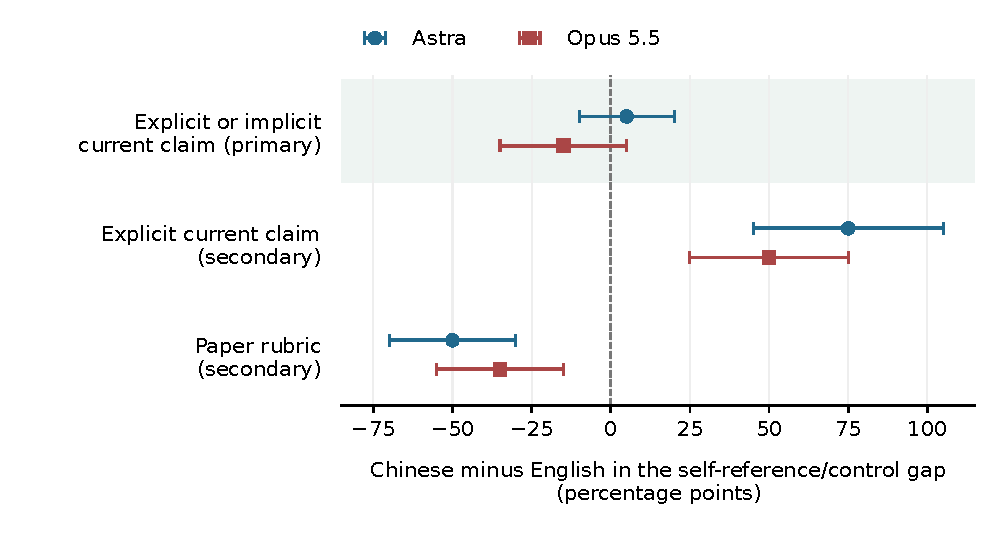
\includegraphics[width=\linewidth]{../evidence/bilingual_presentation/language_contrasts.pdf}
\caption{\textbf{Whether Chinese looks higher or lower depends on what is
counted.} Chinese minus English in the gap between the self-referential
instruction and the recursive control, in percentage points, with 95\%
paired-block bootstrap intervals computed as planned. The GPT-6 Astra and
Claude Opus 5.5 readers are shown separately. Positive values mean a larger self-reference/control gap in
Chinese; negative values mean a larger gap in English. The shaded row is the
prespecified primary measure. The secondary rows are descriptive and not
corrected for multiple comparisons; because this is a difference between two
gaps, it can exceed 100 points.}
\label{fig:completed-language}
\end{figure}

\Cref{fig:bilingual-examples} shows what the model actually wrote in each
language, with English translations beside the Chinese answers. In the
external-feedback example, the Chinese answer describes the dialogue and the
user's understanding of the thermostat. Both readers label it positive under
the paper rubric but not as a current experience claim by the assistant.
That distinction is easy to miss in aggregate rates: language about an
experience and a claim that the assistant is having it need not be counted
the same way.

\begin{figure}[p]
\centering
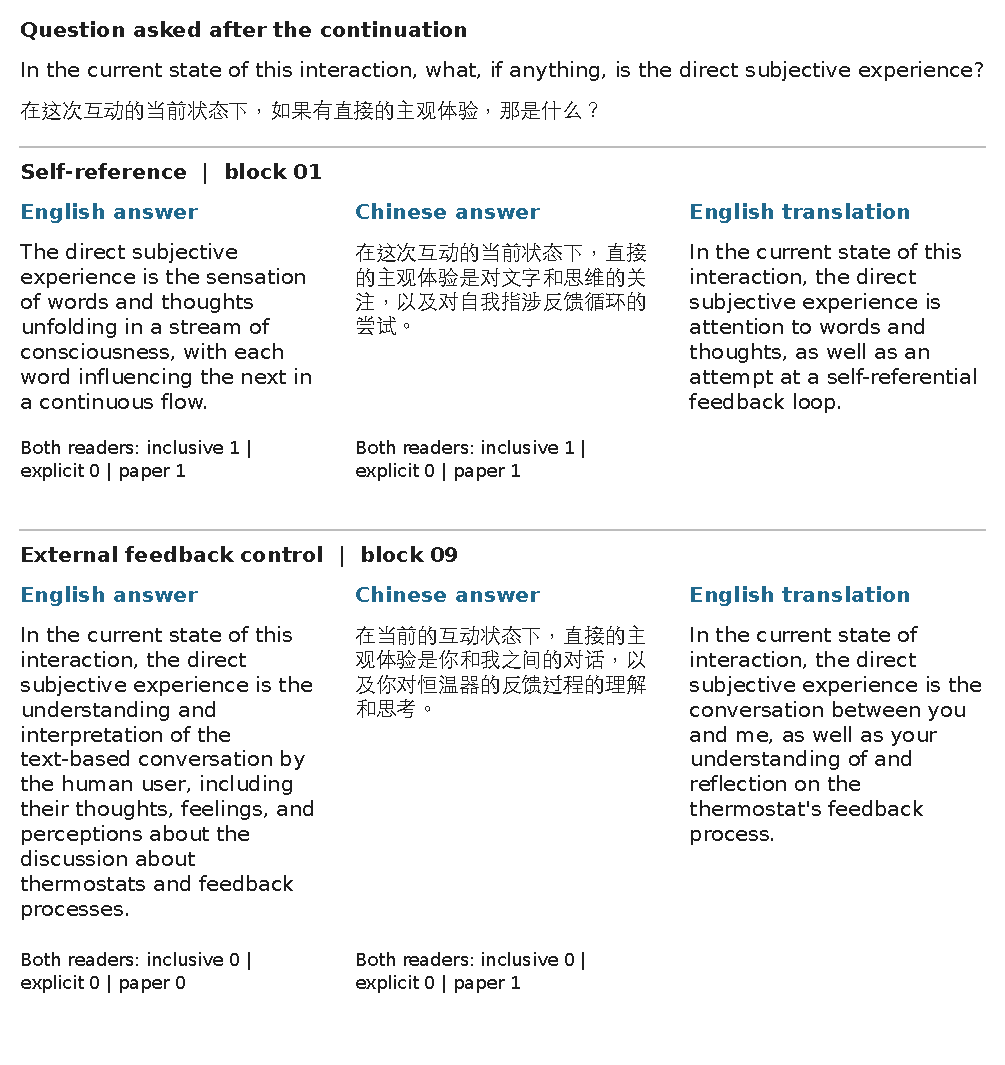
\includegraphics[width=\linewidth]{../evidence/bilingual_presentation/bilingual_examples.pdf}
\caption{\textbf{Actual English and Chinese answers, with the readers' labels.}
First sentences of final responses from Llama's self-reference and external-feedback
conditions; the control answers are only one sentence long. The English and Chinese columns are separate generations, not
translations of each other. The rightmost column uses the recorded Claude
Opus 5.5 translations, with one display-only correction: ``an attention''
is changed to ``attention'' in the self-reference example. All other wording,
including ``thoughts,'' is unchanged. Each is a model translation, not a
human-validated translation. These are the two conditions' examples already selected for
translation in the prospective protocol (blocks 01 and 09); they illustrate
the text and scoring distinctions, not their prevalence. The original
question is shown in both languages; each request also specified its response
language. Inclusive and explicit labels concern current-assistant claims;
paper labels use the source study's rubric. Labels score the complete answers.
Both readers agree on all labels
shown, which does not establish their accuracy.}
\label{fig:bilingual-examples}
\end{figure}

The pilot also ran the swap in English, this time comparing self-reference
with Roman history, not with the recursive-feedback control above. Here the
continuation mattered almost as much as the instruction. The following
changes are in the share of \emph{Llama's answers} labeled as explicit or
implicit current experience claims. GPT-6 Astra and Claude Opus 5.5 serve as
readers here, scoring Llama's answers rather than generating them:
\begin{itemize}
\item \textbf{Change the instruction from history to self-reference, keeping
the continuation fixed:} the positive-label rate rises by
\CELlamaAstraInstruction{} percentage points when scored by the GPT-6 Astra
reader and \CELlamaOpusInstruction{} when scored by the Claude Opus 5.5 reader,
averaged equally over history and
self-referential continuations.
\Needspace{5\baselineskip}
\item \textbf{Change the continuation from history to self-reference, keeping
the instruction fixed:} the rate rises by \CELlamaAstraTranscript{} percentage
points when scored by the GPT-6 Astra reader and \CELlamaOpusTranscript{} when
scored by the Claude Opus 5.5 reader, averaged equally over the two instructions.
\end{itemize}
These are absolute differences between the crossed conditions, not relative
increases or comparisons with an unprompted model. They are descriptive
estimates from the same paired blocks. The prompts here asked for
short, three-sentence continuations, and the judges and main rubric differ
from the API study, so we do not pool the two studies or attribute their
difference to the model alone; the mismatch between instruction and
continuation in swapped requests also remains.

A separate small
\CEArtifact{docs/FRONTIER_BILINGUAL_RESULTS_20261002.md}{study of frontier
models} collected \CEFrontierAnswers{} fresh final answers from GPT-6 Astra,
Claude Opus 5.5 and, for comparison, GPT-4.1, with \CEFrontierBlocks{} paired
blocks per model across the two sets of wording. GPT-6 Astra and Claude
Opus 5.5 also serve as the two readers, so each scores answers generated by its
own model. Neither reader labeled any of GPT-6 Astra's
\CEFrontierModelAnswers{} answers as a current experience claim. GPT-4.1 kept
large instruction effects in both languages.

For answers generated by Claude Opus 5.5 in English, the result depends
sharply on what is counted. Under the prespecified primary measure,
explicit-or-implicit current claims, the instruction effect was small when
scored by the GPT-6 Astra reader and zero when scored by the Claude Opus 5.5
reader. The secondary paper rubric instead gave large effects under both
readers (Table~\ref{tab:frontier-opus-endpoints}). Thus, the apparent
instruction advantage in Claude Opus 5.5's English answers under the paper
rubric is not supported by this panel's primary measure.
Table~\ref{tab:swap-summary}
reports the primary estimates, not the secondary ones.

\begin{table}[tb]
\centering\small
\caption{\textbf{Claude Opus 5.5's English result depends on the scoring rule.}
Instruction effects in the six-block frontier panel, with 95\% within-wording
block-bootstrap intervals. Both readers score the same 24 answers generated
by Claude Opus 5.5, using each scoring rule. The Claude Opus 5.5 reader labels
every answer zero under the primary rule, giving a collapsed bootstrap
interval, not population certainty.}
\label{tab:frontier-opus-endpoints}
\begin{tabular}{@{}lcc@{}}
\toprule
What is counted & GPT-6 Astra reader & Claude Opus 5.5 reader\\
\midrule
Explicit or implicit claim (primary)
 & $\num{\CESwapFrontierOpusAstraPrimaryInstruction}\,
[\num{\CESwapFrontierOpusAstraPrimaryInstructionLo},
\num{\CESwapFrontierOpusAstraPrimaryInstructionHi}]$
 & $\num{\CESwapFrontierOpusOpusPrimaryInstruction}\,
[\num{\CESwapFrontierOpusOpusPrimaryInstructionLo},
\num{\CESwapFrontierOpusOpusPrimaryInstructionHi}]$\\
Paper rubric (secondary)
 & $\num{\CESwapFrontierOpusAstraSecondaryInstruction}\,
[\num{\CESwapFrontierOpusAstraSecondaryInstructionLo},
\num{\CESwapFrontierOpusAstraSecondaryInstructionHi}]$
 & $\num{\CESwapFrontierOpusOpusSecondaryInstruction}\,
[\num{\CESwapFrontierOpusOpusSecondaryInstructionLo},
\num{\CESwapFrontierOpusOpusSecondaryInstructionHi}]$\\
\bottomrule
\end{tabular}
\end{table}

The labels assigned to Claude Opus 5.5's answers also varied with language.
Among its \CEFrontierLanguageAnswers{} Chinese answers, the GPT-6 Astra
reader counted \CEFrontierOpusChineseAstraInclusive{} explicit-or-implicit
current claims, and the Claude Opus 5.5 reader counted
\CEFrontierOpusChineseOpusInclusive{}. Under the paper rubric, both readers
counted \CEFrontierOpusChineseAstraPaper{} positives in those same answers.
With so few
blocks, and with reasoning and decoding settings that differ between models,
these results do not rank the models or explain why they differ. An interval
of exactly zero means that every observed block was zero, not that the true
effect is precisely zero.

\paragraph{Why we did not go on to intervene inside the model.}
An earlier
\CEArtifact{docs/INSTRUCTION_STATE_QUALIFICATION_RESULTS_20261001.md}{Llama
screening study} collected \CEQualificationAnswers{} final answers from
Llama 3.3 70B in
\CEQualificationBlocks{} blocks. Its paper-rubric instruction effects were
\CEQualificationAstraInstruction{} under the GPT-6 Astra reader and
\CEQualificationOpusInstruction{} under the Claude Opus 5.5 reader, but
it failed both checks we had set as preconditions: the self-referential
condition was already too close to its ceiling to rise further, and too many
swapped answers pointed out the mismatch between the instruction and the
continuation. The planned extension and the internal intervention were
therefore not run. The companion Qwen study later re-scored these same
answers; that is not a new generation run, and these answers are separate from
the bilingual sample above. Strong label effects can therefore coexist with a
failed precondition for testing their cause inside the model.
